%% LaTeX2e class for seminar theses
%% seminar.tex
%% 
%% Karlsruhe Institute of Technology
%% Institute for Program Structures and Data Organization
%% Chair for Software Design and Quality (SDQ)
%%
%% Dr.-Ing. Erik Burger
%% burger@kit.edu
%%
%% Version 1.0.1, 2018-04-16

%% Available page modes: oneside, twoside
%% Available languages: english, ngerman
%% Available modes: draft, final (see README)
\documentclass[twoside, english, draft]{Pflichtenheft}

%% ---------------------------------
%% | Information about the thesis  |
%% ---------------------------------

%% Name of the author
\author{PSE GRUPPE}

%% Title (and possibly subtitle) of the thesis
\title{Anomaly Detection in Industrial Networks}

%% Type of the thesis 
% \thesistype{Seminar Thesis}

%% Change the institute here, ``IPD'' is default
 \myinstitute{ KOMPETENZZENTRUM FÜR ANGEWANDTE SICHERHEITSTECHNOLOGIE }

%% The advisors are PhD Students or Postdocs
\advisor{M.Sc. Ankush Meshram}

\settitle

%% --------------------------------
%% | Settings for word separation |
%% --------------------------------

%% Describe separation hints here.
%% For more details, see 
%% http://en.wikibooks.org/wiki/LaTeX/Text_Formatting#Hyphenation
\hyphenation{
% me-ta-mo-del
}

%% --------------------------------
%% | Bibliography                 |
%% --------------------------------

%% Use biber instead of BibTeX, see README
\usepackage[citestyle=numeric,style=numeric,backend=biber]{biblatex}
\addbibresource{pflichtenheft.bib}

\usepackage[nonumberlist]{glossaries}
\makeglossaries

\newglossaryentry{data point}
{
	name=data point,
	plural=data points,
	description={A tuple of values or key-value pairs},
}

\newglossaryentry{data source}
{
	name=data source,
	plural=data sources,
	description={A data source is a service that provides a network interface that can be accessed by the GUI and provides one or more data streams}
}

\newglossaryentry{data stream}
{
	name=data stream,
	plural=data streams,
	description={A sequence of data points. A data stream may grow dynamically, in which case it will provide a kind of "read next" method}
}

\newglossaryentry{diagram}
{
	name=diagram,
	plural=diagrams,
	description={A graphical representation of \glspl{data point} as per a certain \gls{diagram type}. Each data point is represented by a symbol whose position, size, color, shape etc. represent values of the data point. The diagram has labeled axes and, for other properties of the symbol, a legend that allow the user to determine the values represented by each symbol}
}

\newglossaryentry{diagram container}
{
	name=diagram container,
	plural=diagram containers,
	description={The area of the GUI within which the diagram(s) are displayed}
}

\newglossaryentry{diagram type}
{
	name=diagram type,
	plural=diagram types,
	description={A diagram type is a specific style or method of drawing a diagram and visualizing its data points}
}

\newglossaryentry{offline}
{
	name=offline,
	description={a mode in which data is read from the database. Also: data that is read from the database}
}


\newglossaryentry{online}
{
	name=online,
	description={a mode in which data is read from a streaming service or messenger service. Also: data that is read from such a service}
}


\newglossaryentry{role}
{
	name=role,
	plural=roles,
	description={A security role is a list of data sources and diagram types that a user who has this role is allowed to access.}
}


%% ====================================
%% ====================================
%% ||                                ||
%% || Beginning of the main document ||
%% ||                                ||
%% ====================================
%% ====================================
\begin{document}

%% Set PDF metadata
\setpdf

%% Set the title
\maketitle

%% ----------------
%% |   Abstract   |
%% ----------------
 This Document outlines the requirements (both functional and non-functional), environment, target audience, and use cases of the software described below.
%% The text is included from the following files:
%% - sections/abstract

%\begin{abstract}
%\%input{sections/abstract.tex}
%\end{abstract}

\hfill

\begin{center}
    \large{Version 0.5}
\end{center}


%% -----------------
%% |   Main part   |
%% -----------------

\thispagestyle{empty}
\newpage
\thispagestyle{empty}
\tableofcontents
\cleardoublepage
\setcounter{page}{1}


\section{Purpose}\label{sec:intro}
The goal of this project is to create a software visualization tool for industrial network traffic to simplify the analysis of anomalous behaviour, both in realtime and from captured stored data.
\\
This software is part of the ADIN framework and is referered to as the "ADIN Inspector".
\\
One component to achieve this goal is a web interface built with modularity in mind so as to make it easily extendable.
\\
The Web view is able to display a series of diagrams and charts to easily identify the behaviour of the network.
Within the Web view the user has the ability to zoom, select, highlight, and filter out data to better understand the aforementioned behaviour in different OSI layers, as well as visualize the flow rate between network nodes.
\\
To support this Web view a back-end messaging solution is needed. This allows the user to easily switch between multiple streams of captured data.
\\
\section{Overall Description}
While computers can analyze raw data easily, for humans it's easier to recognize behavior using visual aids.
Visual analytics is utilizing graphics to enhance human cognition to understand a problem better or find 'a needle in the haystack' within a huge amount of data. Making it an invaluable tool for security analysis.
\\
Industrial Network Security aims to understand the communication network traffic generated in an industrial production system. Analyzing the traffic generated by underlying industrial protocols is the primary step. 
\\
Real-time visualization of analyzed network data will help the end-user to understand the system's communication behavior and changes within it more clearly. Deviations or incidents can be detected visually by operators as they are occurring or already persisting.
\\
Supplemental to this, the ability of operators to run analysis of past anomalous behavior can help strengthen infrastructure for future failure or attacks. As well as provide useful information for training of new Security analysts.
\section{Interfaces}


	The environment of the project is a modern browser with LAN access. The project is OS-agnostic. Therefore the underlying Operating system is irrelevant on the users end.


\subsection{Software}
\begin{itemize}
\item{Client}
\begin{itemize}
	www-browser of the latest generation.
\end{itemize}
	
\item{Server:}
\begin{itemize}
	\item{Java}
	\item{Kafka messaging framework}
	\item{MongoDB database}
\end{itemize}
\end{itemize}
	
\subsection{Hardware}
\begin{itemize}
\item{Client:}
\begin{itemize}
	System capable of network connectivity
\end{itemize}
	
\item{Server:}
\begin{itemize}
	\item{Network capable system}
	\item{System capable of running all the server-software}
	\item{System with adequate storage}
\end{itemize}

\end{itemize}

\section{Functional Requirements}



\section{Data Requirements}
\section{Non-Functional Requirements}

\begin{description}
  \item[NF100]
  The web UI should be able to visualize the network topology and update the visualization based on real time data streams.
  
  \item[NF110]
  The rendering latency should be no longer than 2 seconds.

  \item[NF120]
  The web UI should be viewable on modern web browsers.

  \item[NF200]
  The framework should be able to handle data streamed from at least $\mathit{N}$ sensors.

  \item[NF210]
  The framework should be able to save data collected in a specified period of time.

  \item[NF300]
  The GUI should be easily extendable with more diagram types.

  \item[NF301]
  The GUI should be easily extendable with more filters and aggregations.

  \item[NF302]
  The GUI should be easily extendable with more data types for input data.

  \item[NF400]
  The system needs to provide access control that authenticates users by using user name and password.

  \item[NF402]
  Each users has one or more security \glspl{role}.

  \item[NF404]
  Multiple users can have the same role.

  \item[NF406]
  A role provides authorization to access certain \glspl{data source} and certain \glspl{diagram type}.

  
\end{description}

\section{Essential Testcases}

\begin{description}
  \item[T100] Successful login
\begin{description}
    \item[Precondition]
    Open browser window.
    \item[Action]
    The user enters the URL for the ADIN webserver in the address bar and presses Enter.
    \item[Reaction]
    The browser loads the ADIN website and shows the login screen.

    \item[Precondition]
    ADIN website had been opened and show the login screen.
    \item[Action]
    The user enters a valid username and the corresponding password.
    \item[Reaction]
    Successfully logged in. The browser loads the ADIN main screen with one empty diagram.
\end{description}

  \item[T102] Failed login (wrong username or wrong password)
\begin{description}
    \item[Precondition]
    Open browser window.
    \item[Action]
    The user enters the URL for the ADIN webserver in the address bar and presses Enter.
    \item[Reaction]
    The browser loads the ADIN website and shows the login screen.

    \item[Precondition]
    ADIN website has been opened and shows the login screen.
    \item[Action]
    The user enters either a valid username and a incorrect password or a nonexisting username and an arbitray password.
    \item[Reaction]
    The login screen shows an error message that the username or password is incorrect and the entry field for the password is cleared.
\end{description}

  \item[T200] Open multiple diagrams.
\begin{description}
    \item[Precondition]
    The browser has been logged in to ADIN and shows the main screen with one empty diagram.
    \item[Action]
    The user presses the "New Diagram" button on the top right side of the screen three times.
    \item[Reaction]
    The browser opens three more diagrams and ends up showing a 2x2 field of four diagrams with the original diagram in the top left position, the second in the top right position, the third in the bottom left position and the fourth in the bottom right position.

\end{description}

\end{description}

\section{Software Modelling}



\subsection{GUI}

The basic data structure needed for graphs are a given set of nodes and a given set of edges, as they are often drawn
as node-link diagrams. In the postal data set, nodes could represent the origins and destinations of postal flows. Edges represent the flows between the respective origins and destinations.In intelligence analysis, investigators use semantic graphs to organise concepts and relationships as graph nodes and links in hopes of discovering key trends, patterns, and insights.” A key issue in graph visualisation is the size of the graph, i.e. the size of the data to visualise. With a growing amount of data to display, graphs can become too complex and overburdening for the analyst’s cognitive capacity. It thus becomes difficult for the user to conduct significant analysis. Because of the issues described above, research often focuses on ways to solve the problems of visual clutter, e.g. by aggregation or clustering techniques, which is also one of the main topics of cartographic generalisation.
\\
In this subsection we'll discuss the GUI, it's components and the workflow of a typical user.
\\
As the programm is opened the user is greeted with a login screen shown in \autoref{fig:loginWindow}. After the user has entered it's credentials and clicked on the login button he is shown \autoref{fig:mainWindow0}.
\\
\vfill

\begin{figure}[h]
\centering
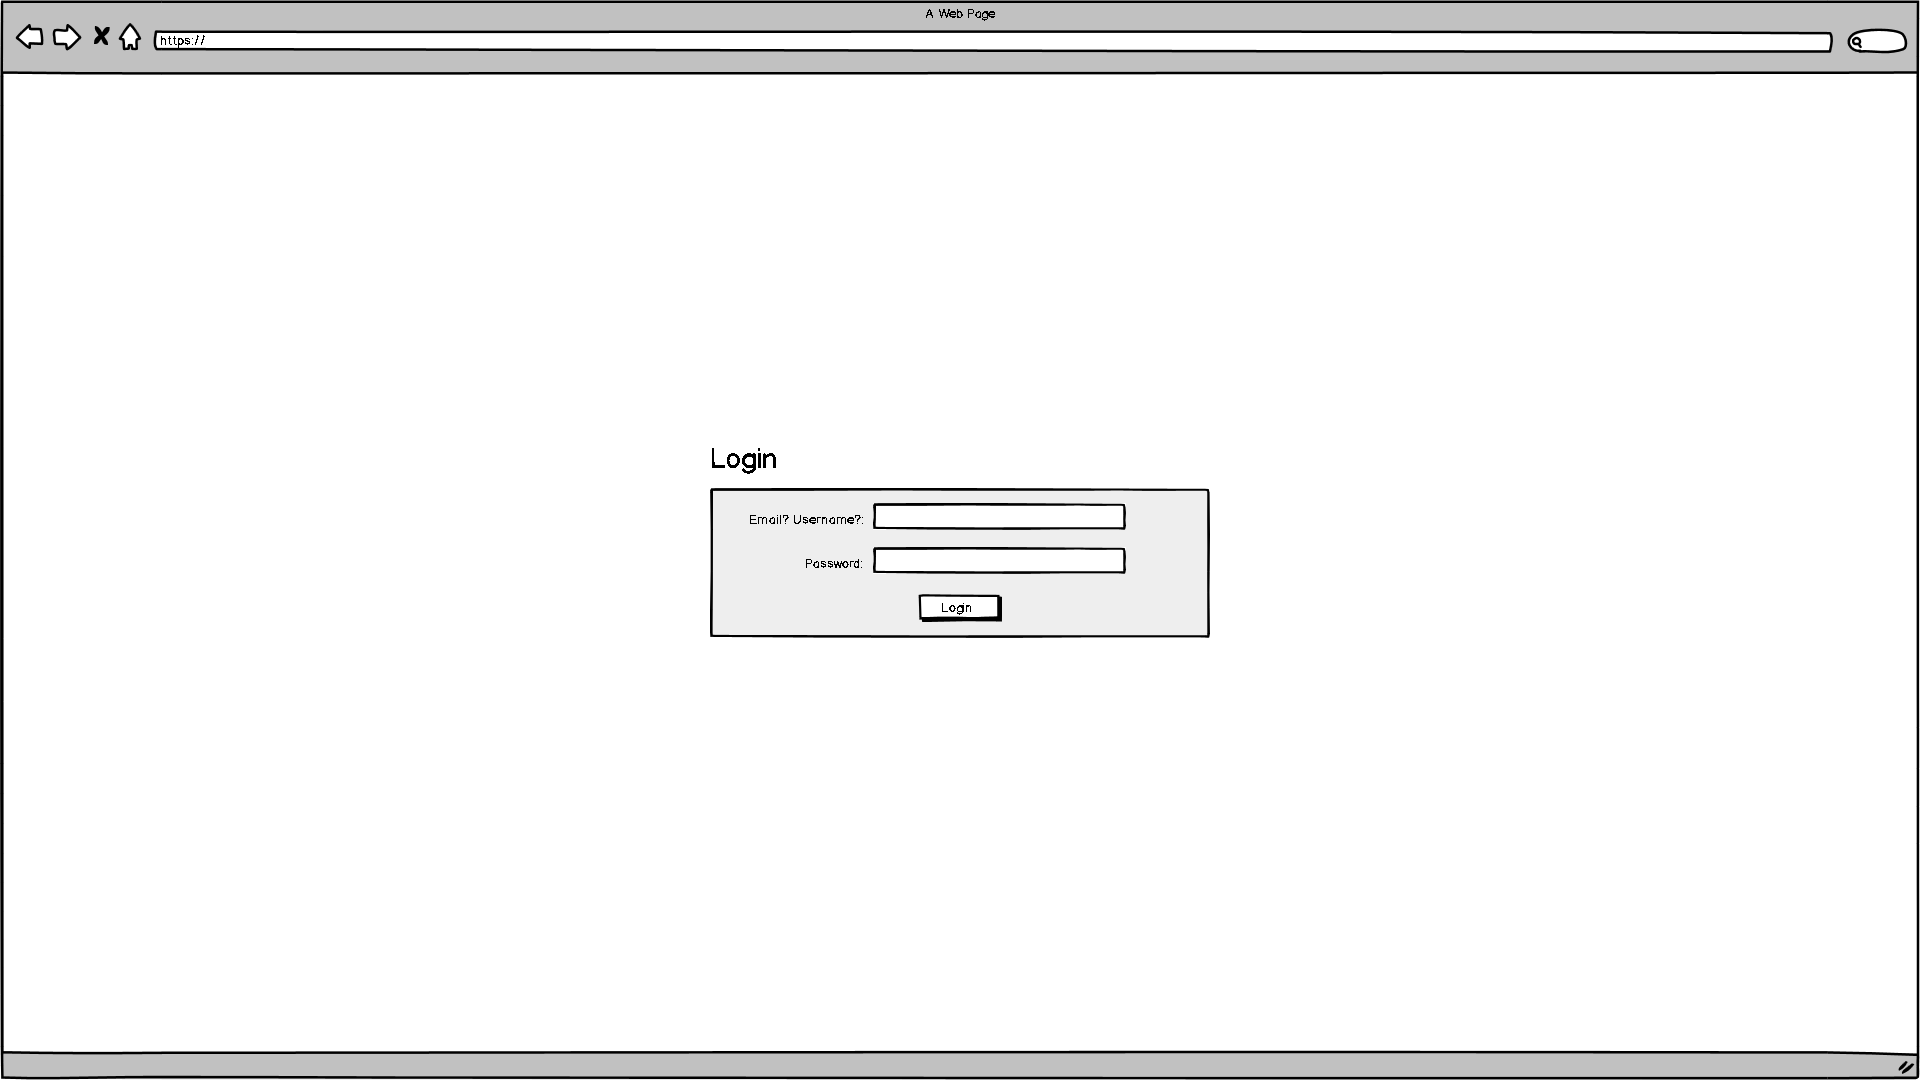
\includegraphics[width=\textwidth]{Images/01MWL.png}
	\caption{The Login Windows shown as the page is first loaded}
	\label{fig:loginWindow}
\end{figure}


\begin{figure}[ht]
\centering
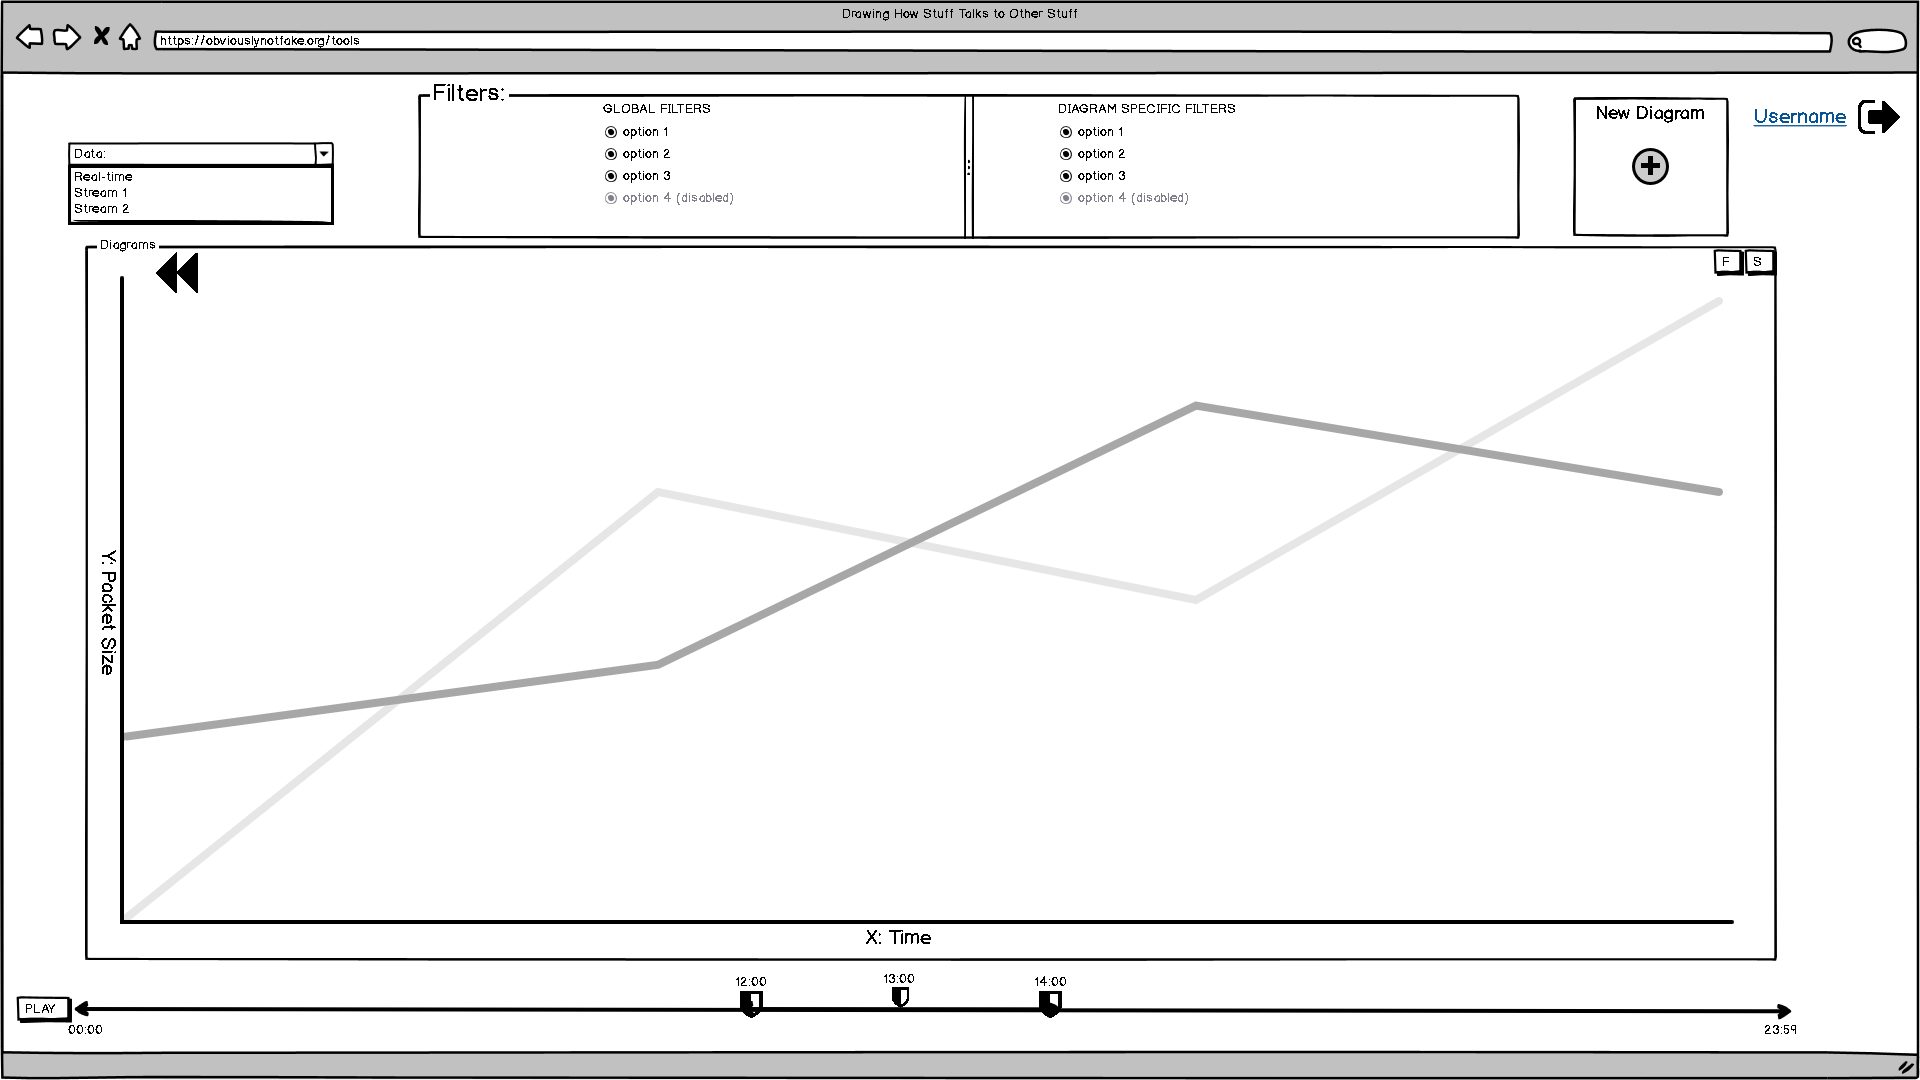
\includegraphics[width=\textwidth]{Images/02MW.png}
	\caption{The Main window the user sees once he logs in}
	\label{fig:mainWindow0}
\end{figure}
\vfill
\clearpage

To discuss in depth this interface it has been divided into subsections labeled in \autoref{fig:mainWindow5}, these are:
\\
\begin{enumerate}
\item The Data stream drop down menu allows the user to select which stream he is currently listening to. This dropdown menu shows the selected diagram selected data stream and by default is set to real-time.
\item Here the user can set filters affecting all diagrams, namely limiting which layers and protocols are currently being shown.
\item Here are the filters being applied to the currently selected diagram, there can further restrict the data being shown globally
\item By clicking this button the user can create a new diagram shown in section 5. The creation workflow is shown in \autoref{fig:mainWindow1} to \autoref{fig:mainWindow5}
\item Here is the currently logged in user, by clicking the button to the right to his name the user can log out.
\item This is the Diagrams container, inside are all diagrams the user has created with all the set constraints. At most 4 diagrams are shown on the container, and more can be made visible via the slider on the right of the container.
\item This is a diagram
\item By hovering with the mouse over a data point a tooltip is shown with all data associated with this data point.
\item These buttons control whether a diagram is fullscreen and the diagram settings. by clicking the button labeled F the diagram grows to take on all available space on the container, like in \autoref{fig:mainWindow0}.
\\
Clicking on the button labeled S replaces the diagram with the Settings for this diagram like in \autoref{fig:mainWindow1}
\item The play button auto scroll along the selected time frame
\item This timeline shows on the left and right bottm labels the beginning and end of all data streams, the labels on top show the currently selected time window and are movable to increase,decrease the time window, the middle shield icon shows the current time while being played, and is also movable to scroll by data manually.

\end{enumerate}


\vfill

\begin{figure}[ht]
\centering
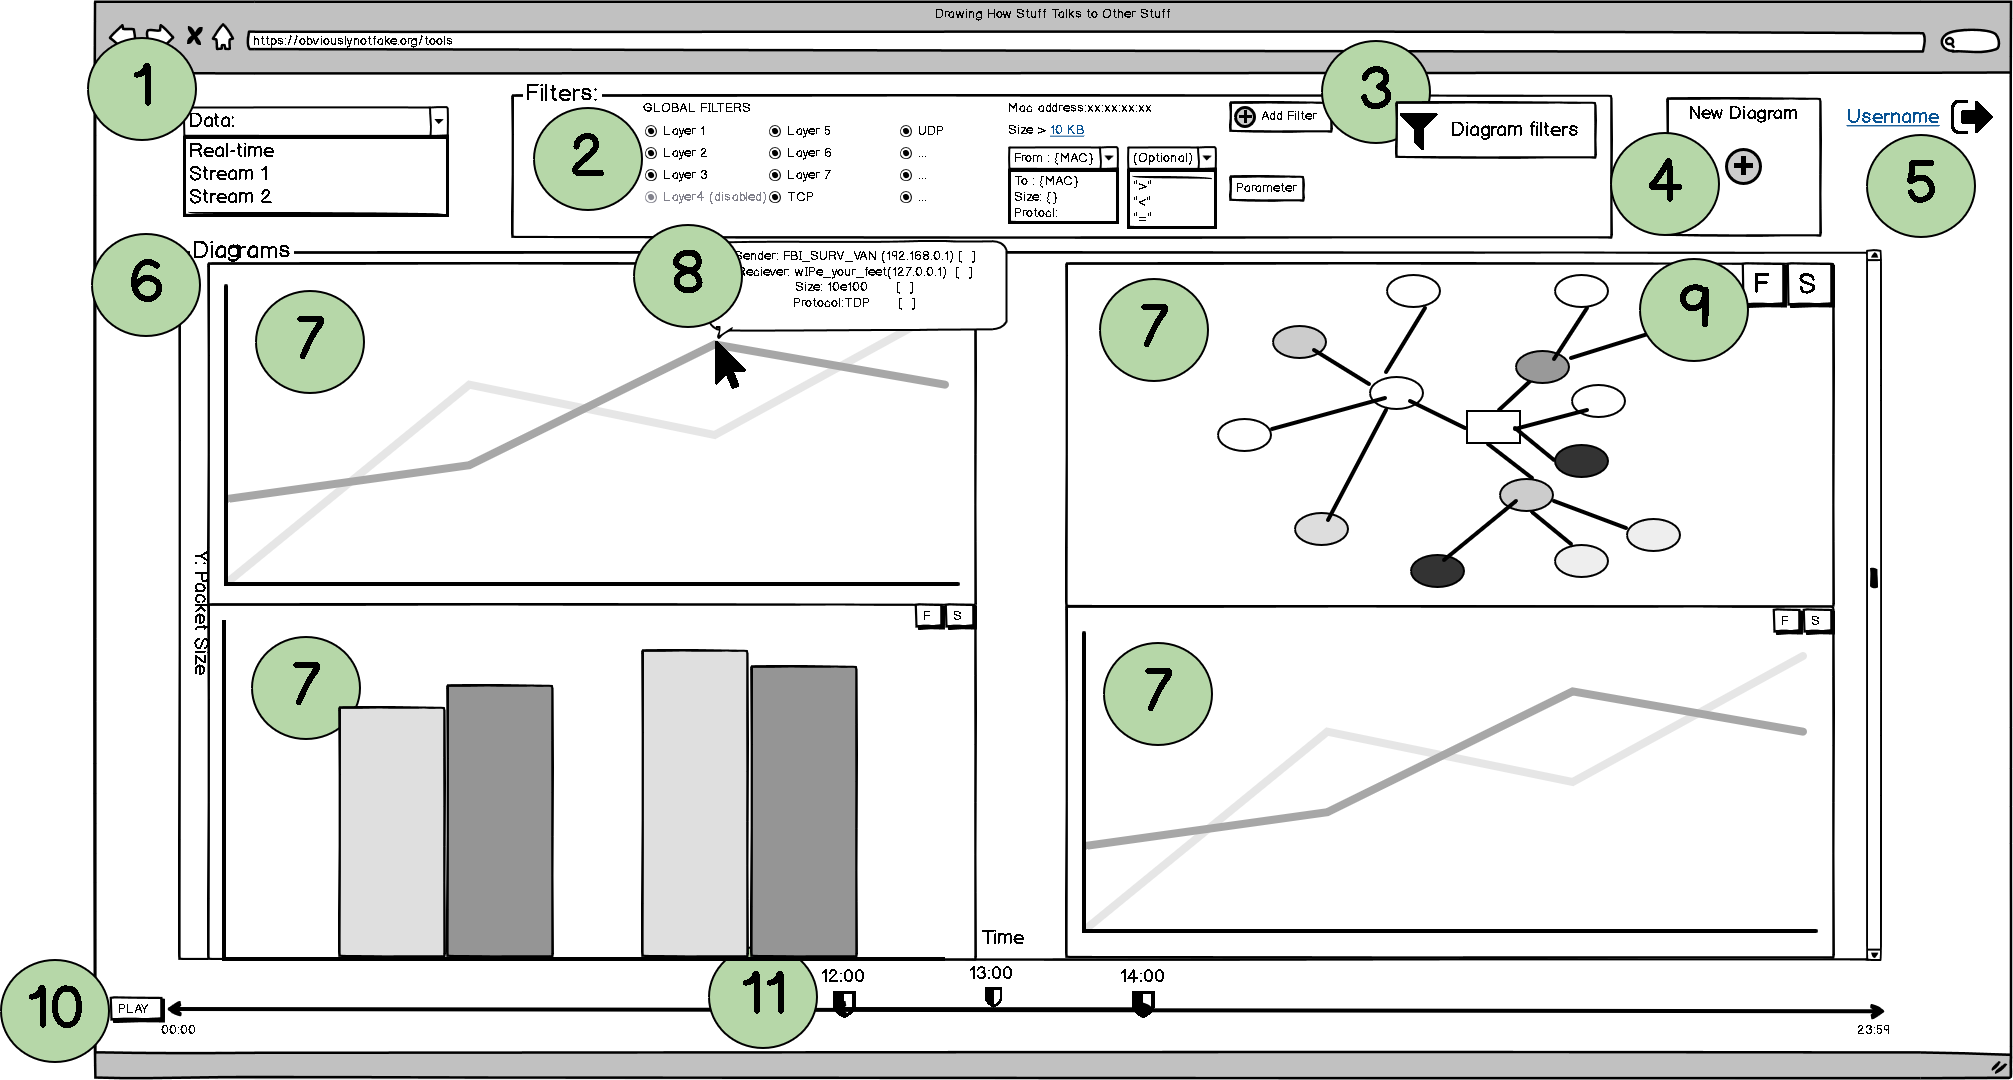
\includegraphics[width=\textwidth]{Images/07MW.png}
	\caption{The GUI divided into relevant sections}
	\label{fig:mainWindow5}
\end{figure}

\vfill
\clearpage

Next we'll take a look at the workflow a user will go through when opening a new diagram.
\\
As referenced above \autoref{fig:mainWindow0} is what the user first sees. When he wants to create a new diagram, by clicking the button labeled new diagram, the Main window is split (shown in \autoref{fig:mainWindow1}) and the new diagram settings are shwon where the new diagram will be.
\\
The user sets here the settings for the new diagram, these are: 
\\
\begin{itemize}
\item{Which data stream it draws its data from}
\item{Which data is pulled to be represented as the x and y axis}
\item{Any filters the user wants to apply at the start}
\end{itemize}

Afterwards, the screen looks like \autoref{fig:mainWindow2}, the diagram container split, by going through this process a two more times the diagram container fills up, containing four diagrams total (shown in \autoref{fig:mainWindow3}), at this point the diagrams have it's minimum size.
\\
Any diagrams created afterwards are spawned underneath the existing ones and the user can scroll up and down to view all of them (shown in \autoref{fig:mainWindow4})

\vfill

\begin{figure}[h]
\centering
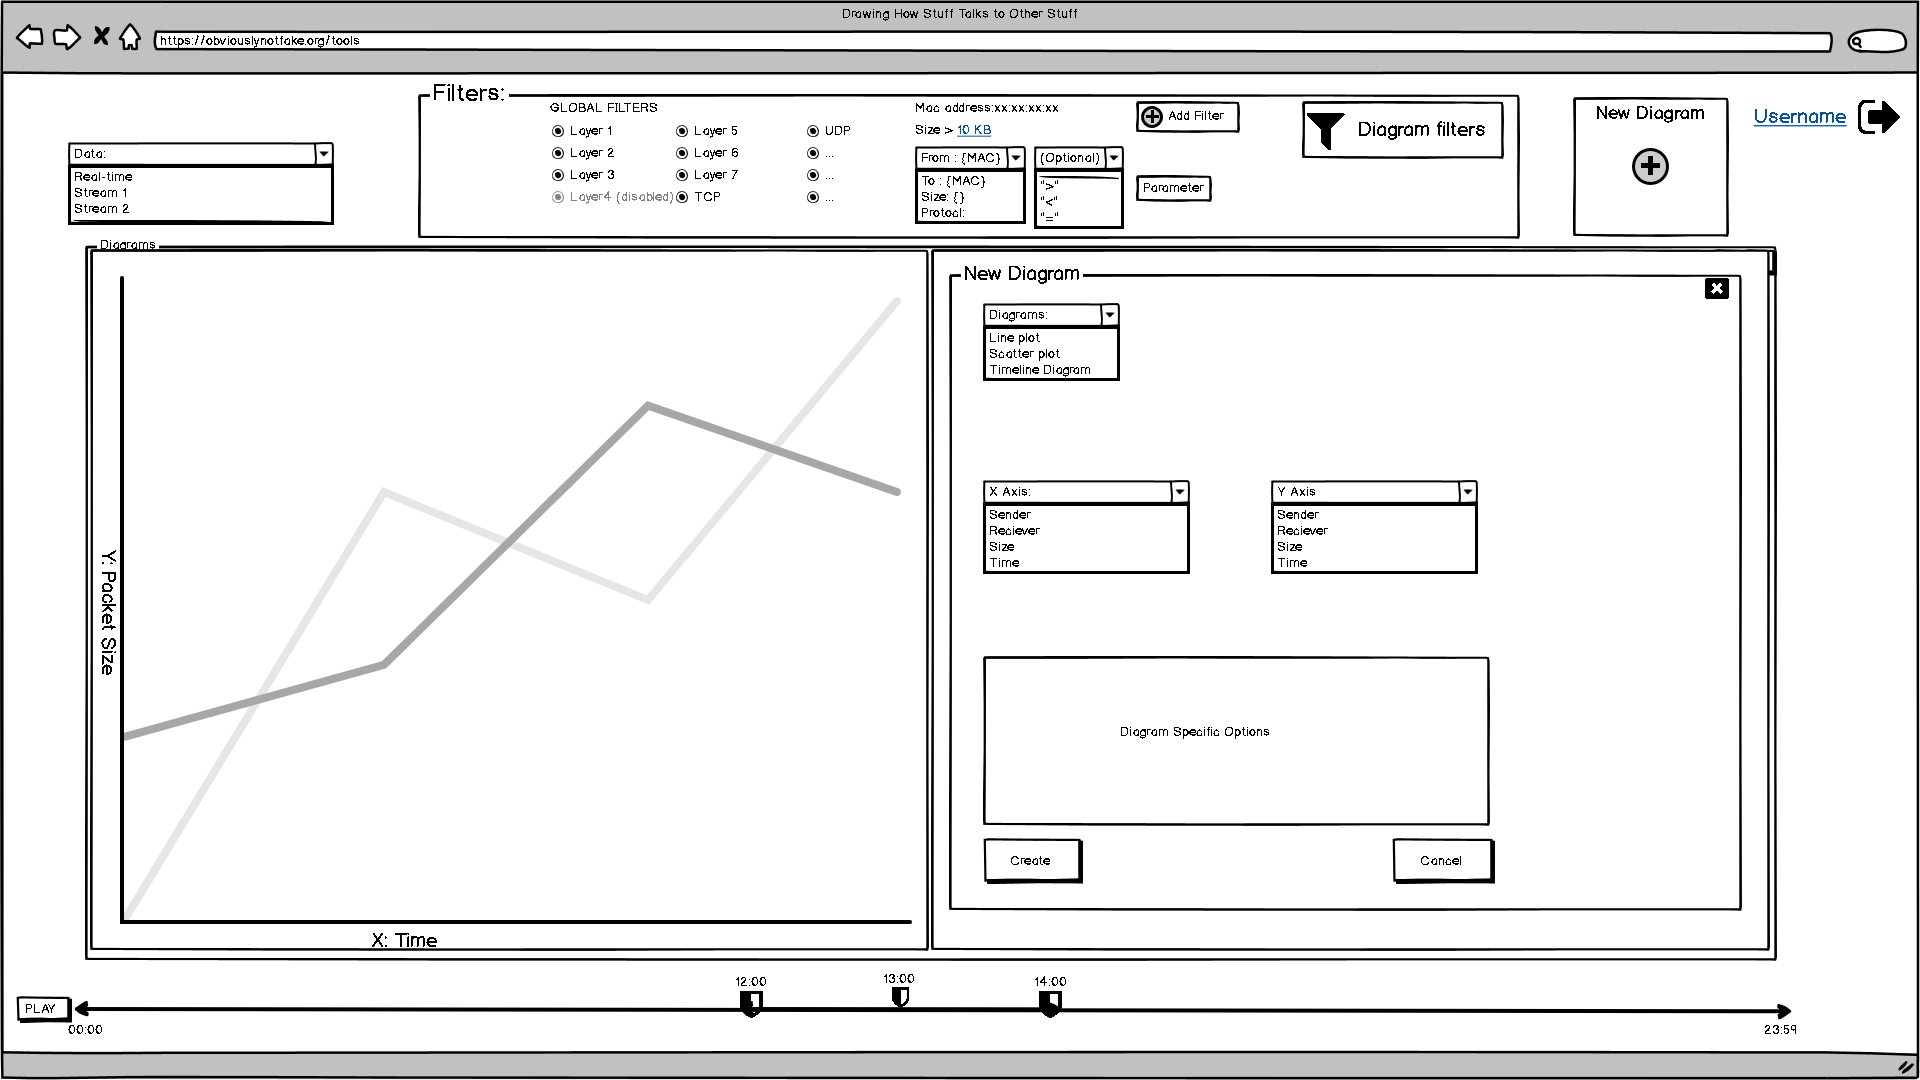
\includegraphics[width=\textwidth]{Images/03MW.png}
	\caption{Main window split in two after user has clicked on the new diagram button. New diagram options are set up on the right.}
	\label{fig:mainWindow1}
\end{figure}


\vfill
\clearpage

TODO:MISSING SECTION ABOUT TOOLTIP FILTERING, NEED TO TALK ABOUT FINAL CHANGES TO THIS!
IMAGES ARE NOT FINAL , STILL UP FOR DEBATE

\begin{figure}[h]
\centering
\label{fig:mainWindow2}
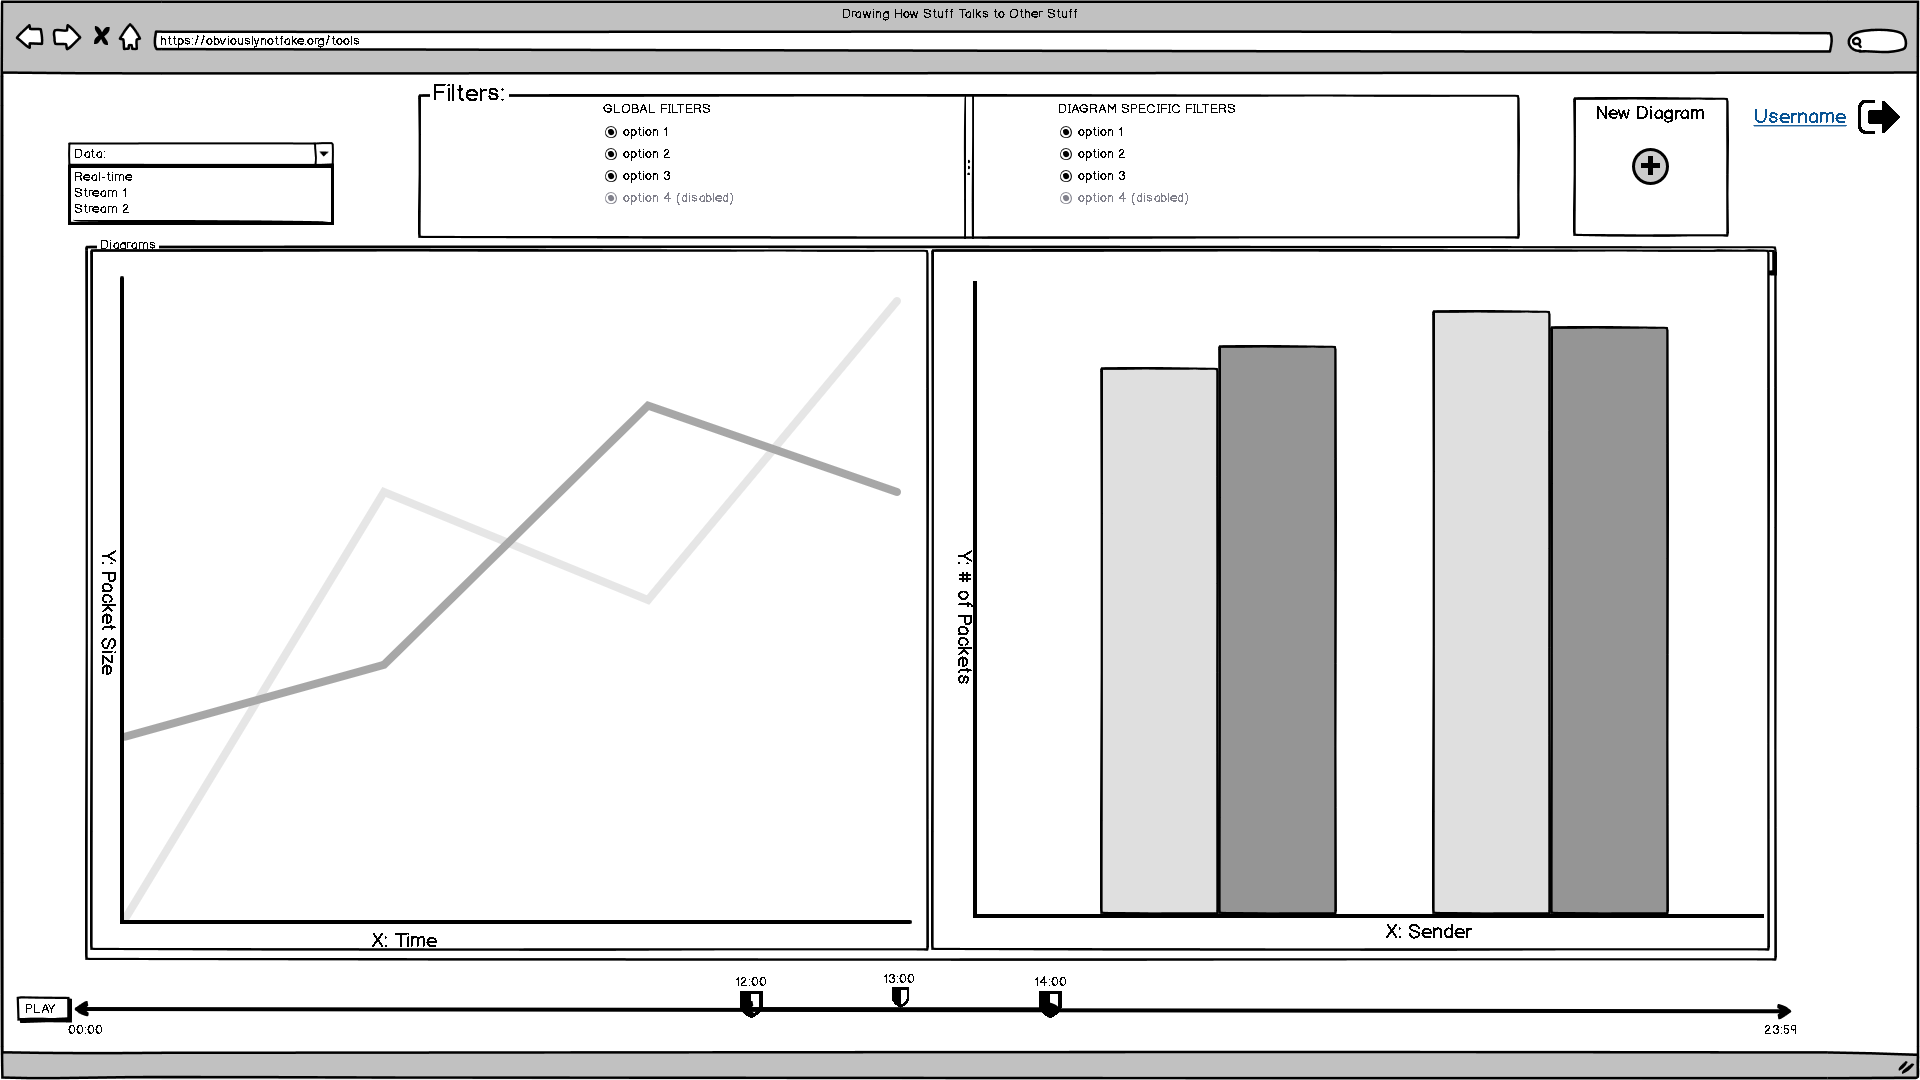
\includegraphics[width=\textwidth]{Images/04MW.png}
	\caption{Main Window with two diagrams side by side.}
		\label{fig:mainWindow2}
\end{figure}



\begin{figure}[h]
\centering
\label{fig:mainWindow3}
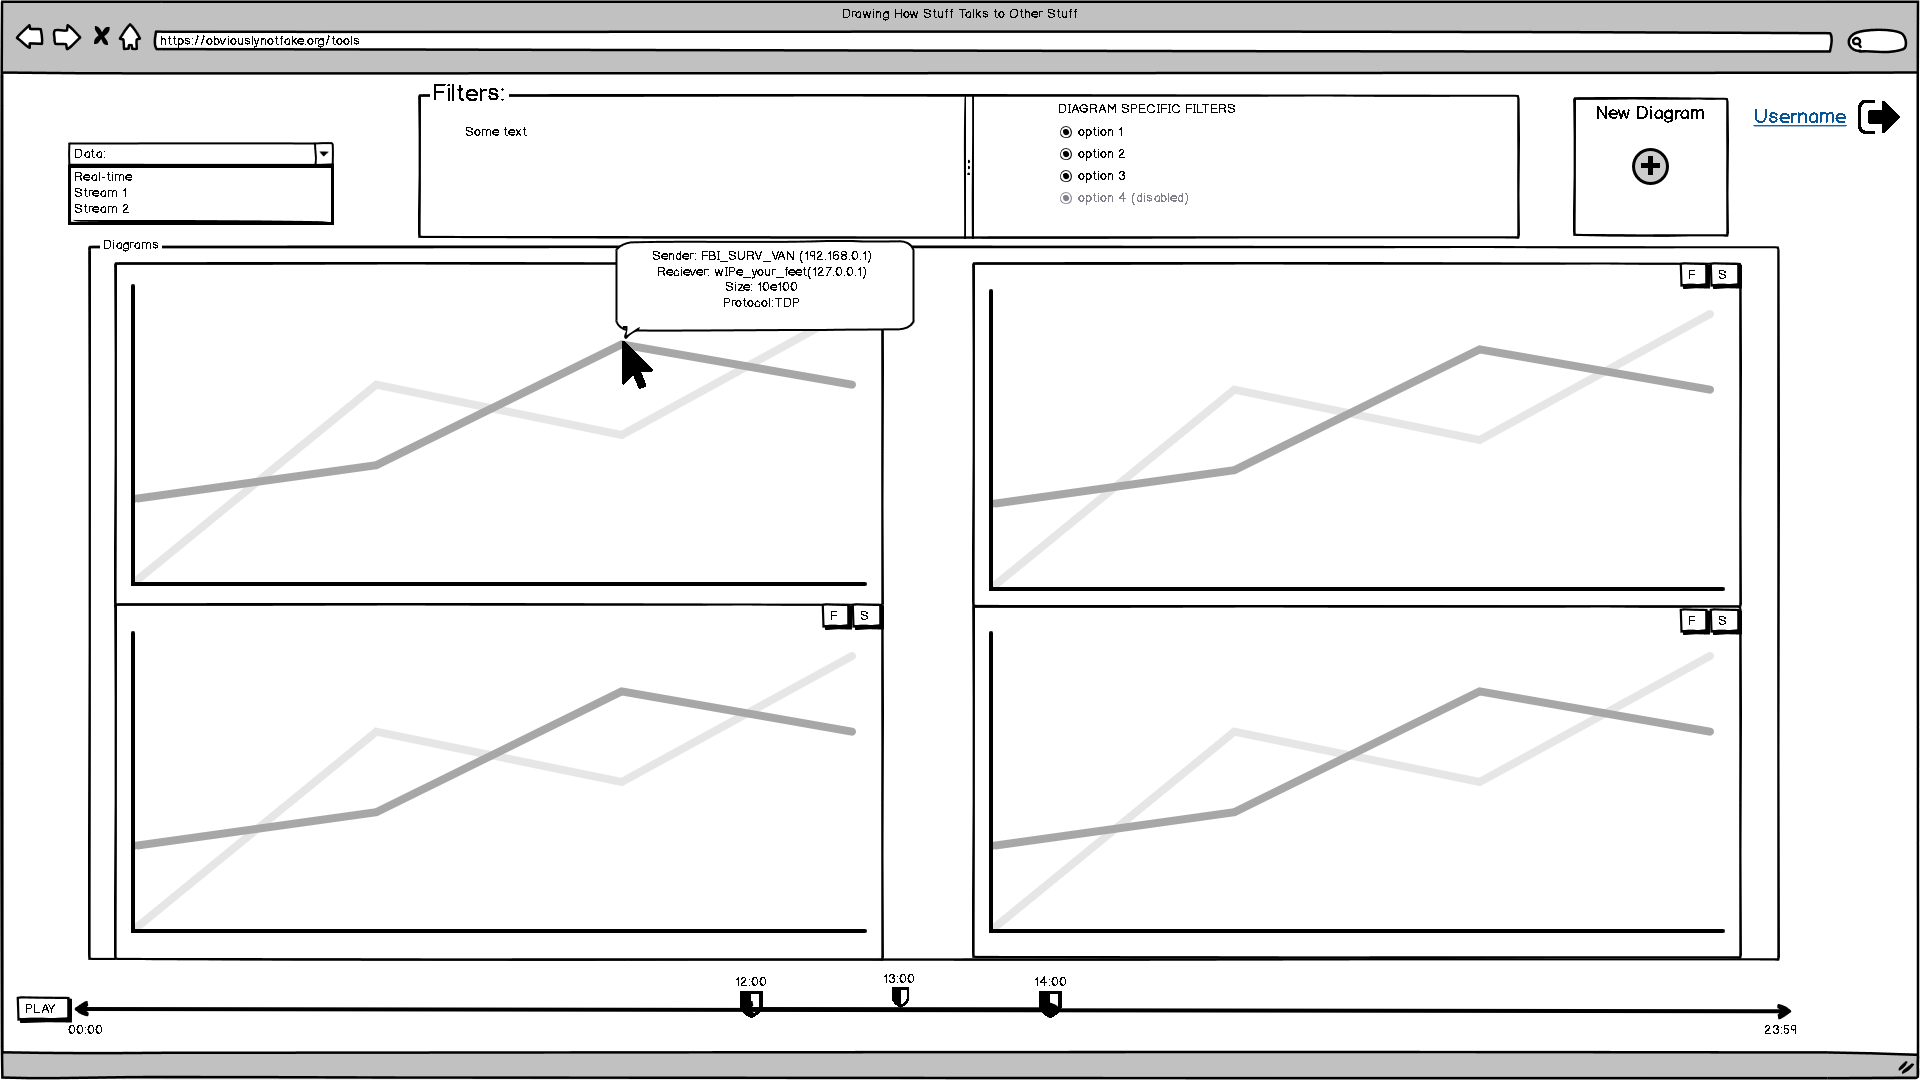
\includegraphics[width=\textwidth]{Images/05MW.png}
	\caption{Main window with four diagrams open}
	\label{fig:mainWindow3}
\end{figure}

\begin{figure}[h]
\centering
\label{fig:mainWindow4}
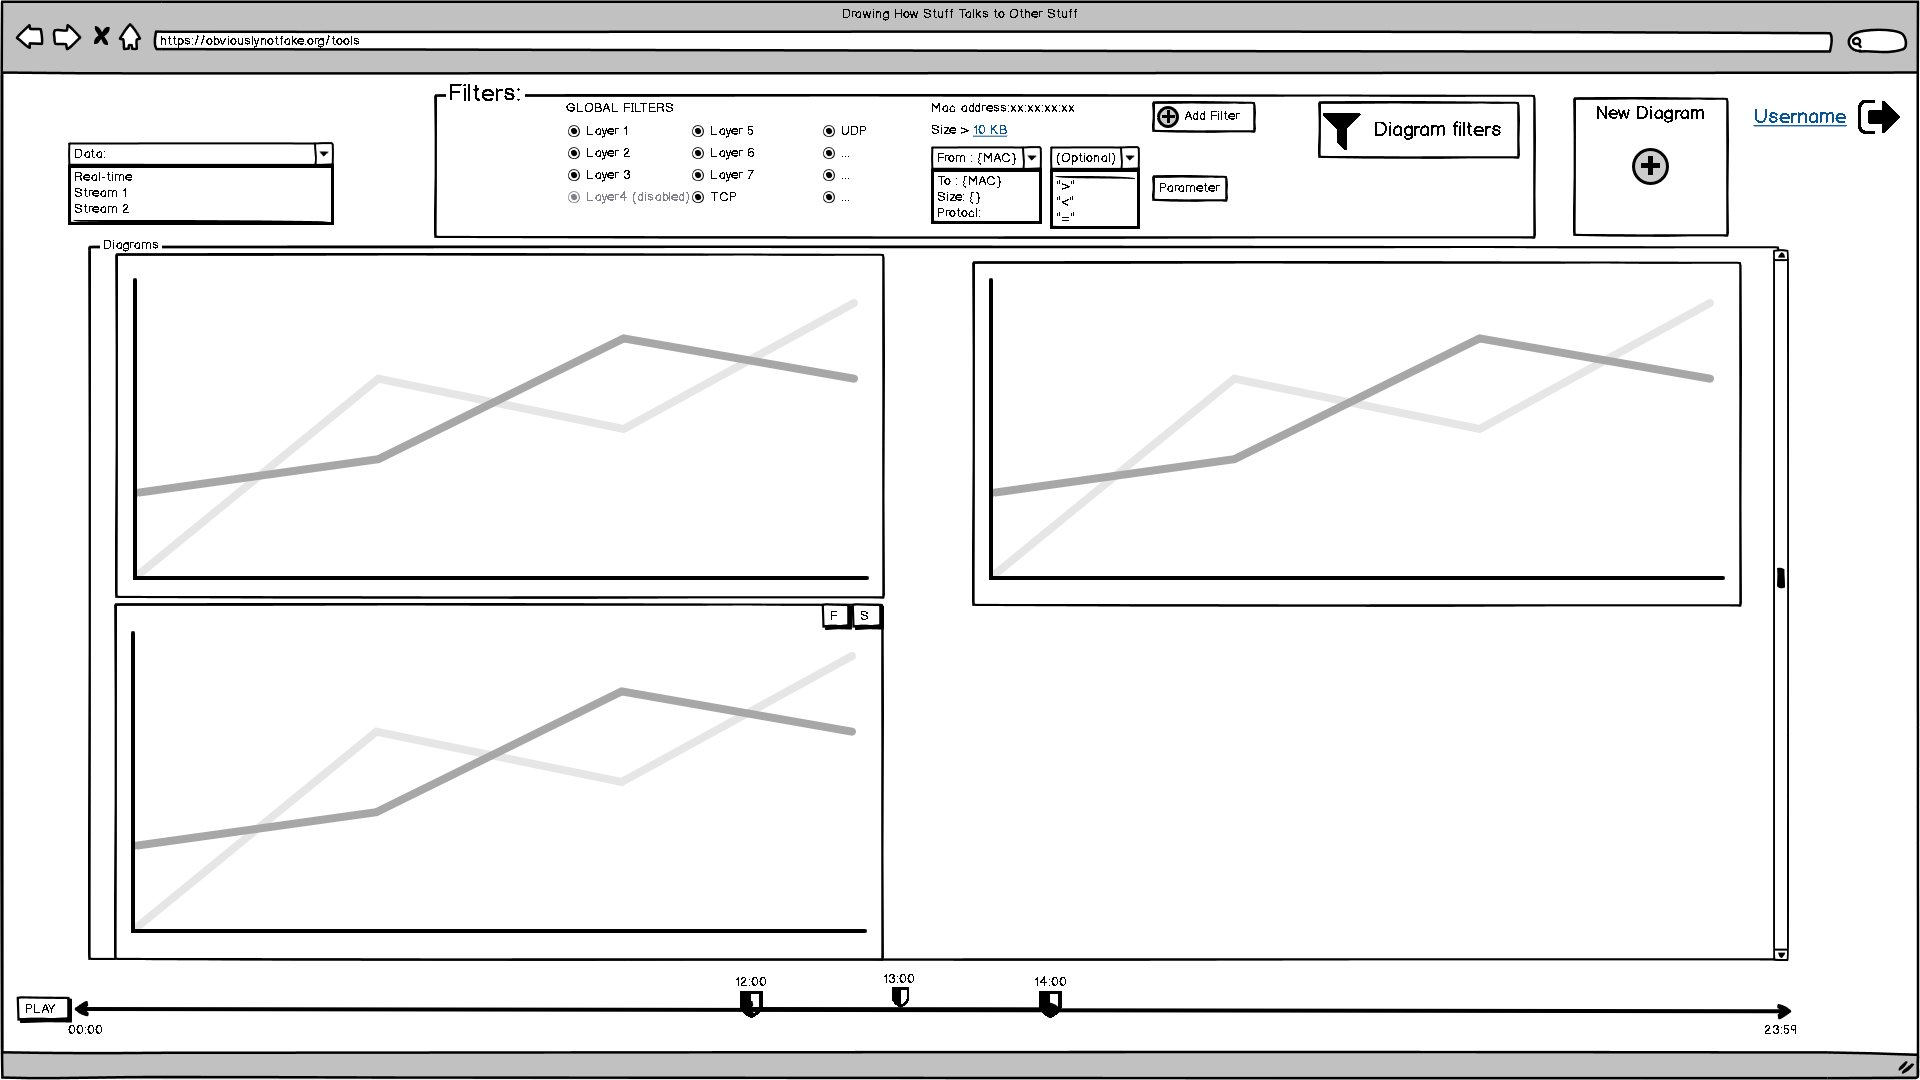
\includegraphics[width=\textwidth]{Images/06MW.png}
	\caption{Main window with more than four diagrams open, more diagrams can be shown using the scroll bar}
	\label{fig:mainWindow4}
\end{figure}

%added this to show all images on GUI section
\clearpage


%%For example, Cui et al. (2008) investigate node-link diagrams for network visualisation.
%Their study focuses on the problem of visual cluttering in graph visualisations,
%as this is one of the main issues in the representation of relationships among
%large data (Herman, Melancon, and Marshall, 2000). They introduce a framework
%for geometry-based edge clustering to group edges into bundles and hence reduce
%visual cluttering caused by the crossing of the high number of edges (see figure 2.1).

\begin{figure}
\centering
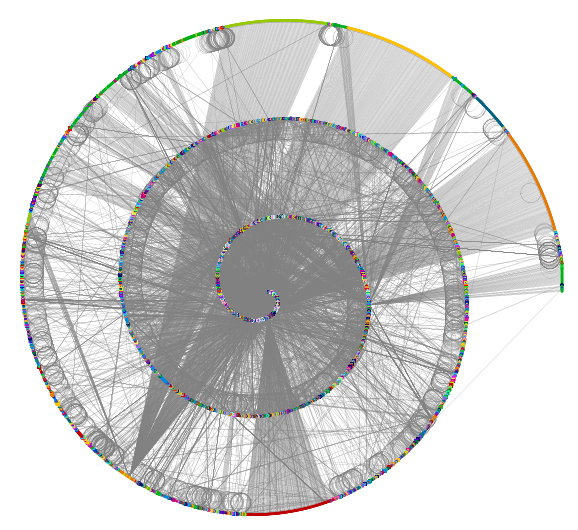
\includegraphics{node.jpg}
  \caption[ height=4cm, width=4cm]{Node-Link-Graph}
\end{figure}



\subsection{Scenario}

\begin{description}
\item[S100:] An operator wants to check manually/visually whether network nodes appeared or disappeared over the last day
\begin{itemize}
\item{the operator opens the web page}
\item{the operator selects the database as data source}
\item{the operator selects a timeline-based \gls{diagram type}}
\item{the operator selects node addresses as the data to be displayed}
\item{the operator moves to or selects the last 24 hours as the range of data to display}
\item{the operator closes the web page}
  \end{itemize}



\item[S200:] A security analyst wants to look at the current flow rates between network nodes to see whether they change / there are trends
\begin{itemize}
\item{the analyst opens the web page}
\item{the analyst selects a source of live data}
\item{the analyst selects an appropriate visualization type}
\item{the analyst selects node addresses as the independent variable}
\item{the analyst selects flow rates as the data to be displayed}
\end{itemize}



\item[S300:] A security analyst wants to examine a specific point of data
\\
Precondition: the analyst has already selected the relevant dataset and visualization type
\begin{itemize}
\item{the analyst selects a data point by right-clicking}
\item{the GUI displays a small pop-up window with all the data of this data point}
\item{the analyst right-clicks one of the attibutes in the pop-up window and selects "Display all corresponding types"}
\item{the GUI marks all data points that have the same value in this attribute}
\end{itemize}



\item[S400:] The user wants to look at alarms/notifications
\begin{itemize}
\item{the user opens the web page}
\item{the user selects the database as data source}
\item{the user selects the data stream from the relevant dissector}
\item{the GUI diplays the notifications along a timeline, according to the time of the event}
\item{the user right-clicks on the x-axis and selects "use record number"}
\item{the GUI diplays the notifications along a timeline adjacently}
\end{itemize}



\item[S500:] The user wants to look at normal data together with alarms/notifications
\\
Precondition: Scenario /S100/ apart from closing the web page
\begin{itemize}
\item{the user selects menu "data", entry "sources"}
\item{the GUI displays a list of all known data sources with a checkbox in front of each}
\item{the user selects the checkboxes for the data sources they want to examine}
\item{the GUI displays data from all these data sources within the currently active visualization}
\end{itemize}


\end{description}

\subsection{Use cases}
\subsubsection{Interactivity}


Visual analytics methods combine interactive visualisations with automated analysis
techniques. This allows the user to decide e.g. which part
of the data he or she wants to explore in more detail.

 A basic principle for visual data exploration was introduced by Shneiderman (1997) by what he called the “The
Visual Information Seeking Mantra: 

Overview first, zoom and filter, then details-ondemand”.
This lets the data analyst define to a certain level what he or she wants
to see and visualise. 

Similar to this, Bertin (1983) specified three “levels of reading,”:
The elementary level (allowing the analyst to look at the information about a
single data record), the intermediate level (showing summarised information about a group of data records), and the global level (providing an overview of all data elements).

\subsection{Object Modelling}
\subsection{Dynamic Modelling}
\subsection{User Interface}

\section{Glossary}
\printglossary[title=,toctitle=]


%% |   Bibliography   |
%% --------------------

%% Add entry to the table of contents for the bibliography
\printbibliography[heading=bibintoc]

\end{document}
